 \hoffset1cm % przesunięcie poziome (przykładowo) o 1cm przeznaczone na oprawę
\documentclass[12pt]{report}
\usepackage[T1]{fontenc}
\usepackage[utf8]{inputenc}
\usepackage{graphicx}
\usepackage{amsmath,amssymb,amsfonts}
%\usepackage{txfonts}
\usepackage{polski}
 
 \usepackage{amsmath}
 \usepackage{amssymb}
 \usepackage{indentfirst}
 \usepackage{listings}
 \usepackage{}
% \usepackage{natbib}
 \usepackage[backend=biber, bibencoding=utf8, style=ieee, isbn=false, doi=false, sorting=anyvt]{biblatex}
%  \bibliographystyle{acm}
 \addbibresource{library.bib}
 \DeclareUnicodeCharacter{229}{ę}
 \DeclareUnicodeCharacter{327}{}
 
 \pagestyle{headings}
 
\renewcommand{\chaptername}{Rozdział}
\renewcommand{\contentsname}{Spis treści}
\renewcommand{\figurename}{Rys.}
\renewcommand{\tablename}{Tab.}
\renewcommand{\listfigurename}{Spis rysunków}
\renewcommand{\listtablename}{Spis tabel}
\renewcommand{\bibname}{Bibliografia}

 \begin{document}

 \begin{titlepage}
 \center{\large\scshape Politechnika Krakowska \\
         \normalsize im. Tadeusza Kościuszki}
 \center{\scshape Wydział Inżynierii Elektrycznej i Komputerowej\\
         Kierunek Informatyka}
 \vspace{0.1\textheight}
 \center{\scshape Michał Patyk}
 \bigskip
 \center{\LARGE\bfseries Sterownik pieca kominkowego, w oprarciu o mikrokontroler (lub platformę komputerową), zgodny ze szkicem specyfikacji Web Thing API}
 \center{(praca inżynierska)}
 \vspace{0.3\textheight}
 \par
 \rightline{Promotor: Dr Radosław Czarnecki}

 \vspace{0.1\textheight}
 \center{Kraków 2020}
 \end{titlepage}


 \tableofcontents


 \chapter{Wstęp}
% \addcontentsline{toc}{chapter}{Wstęp}
dodaj wykres popularności źródeł w czasie
 \section{Rys historyczny - ujęcie problemowe}
 Problem ogrzewania pomieszczeń towarzyszy człowiekowi od zarania dziejów. Zwykle był to proces wymagający ciągłego nadzoru. Potrzeba automatyzacji wydaje się naturalną konsekwencją zmiany trybu życia człowieka. Wraz z pojawieniem się nowoczesnych kotłów powstały pierwsze mechanizmy kontrolujące pracę urządzenia bez nieustannej koniecznosci doglądania go.
 Pojawienie się sterowników cyfrowych zaoferowało zupełnie nowe możliwości, takie jak:
  \begin{enumerate}
 \item[•] większą efektywność pracy systemu grzewczego
 \item[•] zmniejszenie emitowanych zanieczyszczeń
 \item[•] wzrost komfortu użytkowania
 \item[•] poprawę bezpieczeństwa
 \item[•] w nowszych modelach - zdalne sterowanie
  \end{enumerate}
 Sterowniki cyfrowe wydają się również odpowiedzią na coraz bardziej dostrzegany problem odpowiedzialnego wykorzystywania zasobów naturalnych, gdyż za ich pomocą do zapewnienia komfortu termicznego pomieszczeń potrzebna jest znacznie mniejsza ilość paliwa. Stanowią one również propozycję rozwiązania problemu ubóstwa energetycznego.
 
 \section{Stan aktualnej wiedzy}
 Obecnie na rynku dostepny jest szeroki wachlarz rozwiązań, od prostych jednokomponentowych do bardziej zaawansownach, złozonych. Począwszy od regulatorów pokojowych, które jedynie włączają ogrzewanie kiedy temperatura pomieszczenia obniży się ponizej nastawionej wartości, poprzez rozbudowane, umożliwiające programowanie temperatury zarówno w ciągu doby (nizsza w nocy, wyższa po południu), jak i w wybrane dni tygodnia, skończywszy na automatyce pogodowej, która dzięki wykorzystaniu czujnika zewnętrznego, umieszczonego na ścianie domu, przewiduje zwiększone zapotrzebowanie na ciepło i wcześniej dostosowuje moc kotła.
 Coraz więcej dostępnych na rynku sterowników umożliwia zdalne nastawienie temperatury. W znakomitej większości standard komunikacji tych rozwiązań jest zamknięty, co utrudnia współpracę  z innymi inteligentnymi urządzeniami.
 
 \section{Innowacyjność projektu na tle współczesnych rozwiązań}
 W odróżnieniu od szeroko stosowanych rozwiązań mój projekt zakłada użycie specyfikacji Web Thing API \cite{Mazurek2018}, która pozwala na ujednolicenie dostępu do inteligentnych rzeczy za pomocą dodatkowej warstwy abstrakcji. Oznacza to, że system kreuje przestrzeń kooperacji urządzeń. Możliwe interakcje wpływają pozytywnie na koherentność systemu.
 
 \section{Motywacje}
Pomysł na pracę zrodził się z potrzeby zmniejszenia ilości czasu oraz poświęcanej uwagi potrzebnych do obsługi pieca kominkowego, pracującego jako główne źródło ciepła w domu jednorodzinnym. Ponadto niekomfortowym ograniczeniem dotychczas stosowanych rozwiązań jest zmuszanie klienta do użytkowania produktów pochodzących od tego samego producenta, co w znaczącym stopniu ogranicza możliwość wyboru preferowanego sprzętu.


 \chapter{Cele pracy, zakres pracy, założenia}

 \section{Cele pracy}
 Celem niniejszej pracy jest \textbf{opracowanie koncepcji sterownika pieca kominkowego} zgodnego ze szkicem specyfikacji Web Thing API.
 
 \section{Zakres pracy}
 Zakres pracy obejmuje:
 \begin{enumerate}
 \item przegląd istniejących rozwiązań - zarówno sprzętowych jak i programowych; (komputerowe systemy sterowania, inżynieria systemów informacyjnnch)
 \item opracowanie koncepcji; (komputerowe systemy sterowania, mikroprocesory i mikrokontrolery, systemy operacyjne)
 \item wybór podzespołów; (architektura systemów komputerowych, podstawy elektroniki i techniki cyfrowej, mikroprocesory i mikrokontrolery, systemy wbudowane)
 \item wykonanie prototypu na płytce stykowej; (systemy wbudowane)
 \item stworzenie oprogramowania; (symulacja komputerowa, systemy wbudowane, technologie obiektowe, programowanie obiektowe, sieci komputerowe)
 \item przetestowanie oprogramowania; (systemy odporne na błędy)
 \item zaprojektowanie płytki drukowanej - PCB; (elektrotechnika, podstawy elektroniki i techniki cyfrowej)
 \item zaprojektowanie obudowy
 \item zintegrowanie z Mozilla Gateway
 \item przygotowanie instrukcji obsługi
 \end{enumerate}
 
 \section{Założenia i wymagania}
 
 Wykorzystane narzędzia:
 \begin{enumerate}
 \item[•] środowisko programistyczne CLion
 \item[•] język programowania C/C++
 \item[•] ekosystem PlatformIO
 \item[•] oprogramowanie do projektowania PCB KiCad
 \item[•] platforma monitoringu i kontroli urządzeń WebThing Mozilla
 \item[•] wzorzec projektowy - \dots
 \end{enumerate}
 
 Sterownik ma umożliwić:
 \begin{enumerate}
 \item[•] monitorowanie pracy pieca kominkowego
 \item[•] lokalne i zdalne zadawanie temperatur
 \item[•] informowanie o zdarzeniach
 \end{enumerate}
 
 Wymagania:
 \begin{enumerate}
 \item[•] zgodność z Web Thing API
 \item[•] watchdog
 \item[•] możliwość rozbudowy o dodatkowe czujniki i elementy wykonawcze
 \item[•] przywracanie nastaw po utracie zasilania
 \item[•] zamknięcie dolotu powietrza na czas dokładania paliwa
 \item[•] minimalizacja otwarcia przepustnicy w przypadku zaniku napięcia
 \item[•] sygnalizacja uszkodzenia czujnika temperatury
 \item[•] regulowana jasność wyświetlacza - zwiększana na czas zmiany ustawień (opcja)
 \item[•] sygnalizator dźwiękowy który informuje gdy temperatura wzrośnie do niebezpiecznego poziomu
 \end{enumerate}
 
 \section{Efekt końcowy}
 Planowanym efektem końcowym pracy będzie stworzenie sterownika pieca kominkowego, pozwalającego na bezobsługową pracę paleniska pomiędzy momentami uzupełniania paliwa.

 Element wyróżniający wykonany sterownik stanowi wykorzystanie Web Thing REST API, który pozwala na wykorzystanie sieci jako zunifikowanej warstwy abstrakcji dla zdecentralizowanego internetu rzeczy.
 
 Rysunek~\ref{fig:wizja} na stronie~\pageref{fig:wizja} przedstawia wizję struktury elementów sterownika
 \begin{figure}[ht]
\centering
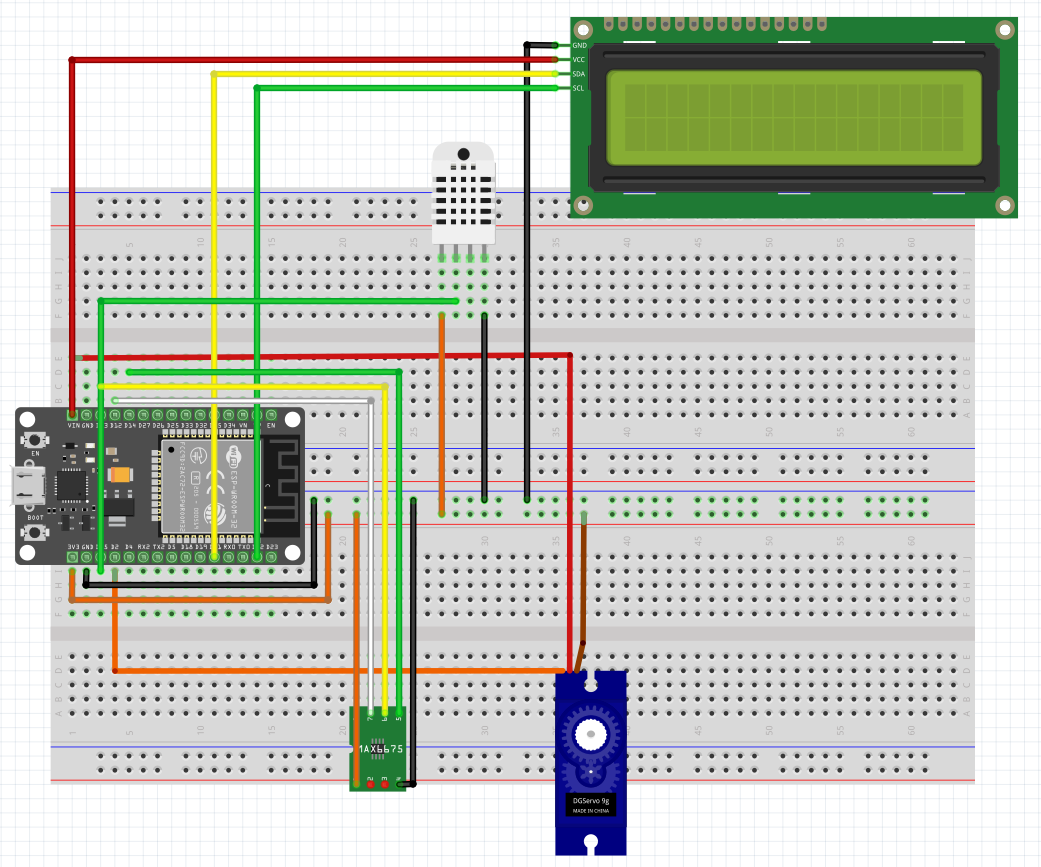
\includegraphics[width=0.8 \textwidth]{fig/fritzing_bredboard_v1.png}
\caption{Wizja elementów sterownika. Opracowanie własne.}
\label{fig:wizja}
\end{figure}
 
 \section{Dalsze kierunki rozwoju}
 W tej części zostaną opisane możliwe kierunki rozwoju sterownika.
 
 Integracja z systemem odzyskiwania ciepła ze spalin.
 Zmiana frameworka z Arduino na Espressif IoT Development Framework - bardziej profesjonalne rozwiązanie, lepsza współpraca z mikrokontrolerem.
 \ldots
 

 \chapter{Charakterystyka metod obsługi} 
 Obsługa w pełni manualna wymaga stałego nadzoru nad przebiegiem spalania. Jest bardzo absorbująca. Łatwo prowadzi do przekroczenia pożądanych temperatur. Pogarsza efektywność procesu spalania, co prowadzi do obniżenia ogónej sprawności kotła, większego zapotrzebowania na opał, a w konsekwencji znacznie wyższych kosztów ogrzewania.
 
 Obsługa półautomatyczna pozwala na samodzielną pracę urządzenia pomiędzy momentami dokładania paliwa. Można wyróżnić dwie jej odsłony. Mechaniczna, w której głowica termostatyczna połączona jest z mechanizmem dźwigni. Na jej ramieniu znajduje się łańcuszek lub linka. Zaletą jest niski koszt. Elektroniczna, gdzie stosuje się sterownik pokojowy z serwomechanizmem. Koszt tego rozwiązania jest umiarkowany oraz zapewnia szerokie możliwości regulacji, umożliwiając dokonywanie nastaw lokalnie lub zdalnie.
 
 Najdroższe jak i najbardziej autonomiczne rozwiązanie stanowi obsługa automatyczna, w której kocioł z podajnikiem paliwa pracuje samodzielnie do kilku dni
 
 
 \chapter{Przegląd istniejących rozwiązań} 
 \section{Standardy integracji inteligentnych urządzeń}
 Zamiast wymyślac kompletnie nowe standardy, Web of Things wykorzystuje istniejące, dobrze znane standardy webowe.
  
 \section{Sterowniki kominkowe}
 Na rynku istnieje szeroka gama rozwiązań przeznaczonych do kotłów na paliwo stałe, jednak stosunkowo niewielka ilość sterowników przeznaczonych dla kominków. - tylko z dodatkową przepustnicą co ogranicza możliwość regulacji (powietrze pierwotne i wtórne).
 \subsection{TECH STEROWNIKI}
 Firma TECH ma w swojej aktualnej ofercie \cite{Tech} trzy sterowniki do kominków. Dwa znich są do kominków z płaszczem wodnym. Trzeci \cite{TechSterownik} przeznaczony jest do kominków z dystrybucją gorącego powietrza i mógłby zostać zastosowany przy piecu kominkowym. Czujnik mierzy temperaturę spalin.
 Aby mieć możliwość zdalnego dostępu do sterownika należy skorzystać z jednego z dwóch dodatkowych modułów komunikacyjnych - GSM lub Ethernet. Dosęp jest możliwy jedynie przez stronę producenta lub aplikację mobilną, brak publicznego API.
 Sam moduł Ethernet kosztuje około 500zł \cite{TechEthernetCena}.
 \subsection{EUROSTER}
 Firma EUROSTER ma w swojej aktualnej ofercie \cite{Euroster} tylko jeden seteronik do kominków. Jest on \cite{EurosterSterownik} przeznaczony do współpracy z kominkiem z płaszczem wodnym więc nie może być zastosowany do pieca kominkowego. Nie posiada możliwości zdalnego dostępu. Czujnik mierzy temperaturę wody obiegowej.
 Cena samego sterownika to około 300zł \cite{EurosterSterownikCena}. Dodatkowo należy zakupić przepustnicę.
 \subsection{Kratki}
 Firma Kratki ma w swoje ofercie \cite{Kratki} jeden sterownik do kominków występującwy w kilku wersjach różniących sie obudową i wielkością dołączonej do zestawu przepustnicy.
 Jest on przeznaczony do współpracy z kominkami każdego rodzaju dlatego może zostac zastosowany do pieca kominkowego. Nie posiada możliwości zdalnego dostępu. Czujnik miezy temperaturę w pobliżu paleniska. 
 Cena samego sterownika to około 400zł \cite{KratkiSterownik}.
  \subsection{Podsumowanie}
  Tylko jeden z wymienionych producentów pozwala na zdalny dostęp do sterownika, jednak jest on tylko możliwy za pośrednictwem serwerów producenta. Brak publicznego API. Cena tego rozwiązania jest wysoka.
  Tylko jeden z wymienionych sterowników posiada czujnik pozwalający na mierzenie temperatury spalin.
  
  
 \chapter{Opracowanie koncepcji}
 Regulacja dopływu powietrza do komory spalania. Jak dobrać otwarcie przepustnicy? Pomiar temperatury spalin.
 W minimalnej wersji: pomiar temperatury spalin i dobranie otwarcia przepustnicy. Potrzebne tylko mikrokontroler, serwo oraz termopara.
 Dodatki:
 \begin{enumerate}
 \item termometr mierzący temperaturę w pomieszczeniu aby zwiększać moc przy większym zapotrzebowaniu na energię
 \item wyświetlacz przekazujący informacje użytkownikowi
 \item wyjście sterujące wentylatorem wymuszający obieg powietrza do innych pomieszczeń dla lepszej dystrybucji energii
 \item czujnik otwarcia drzwi paleniska aby zmieniać parametry pracy po dołożeniu drewna
 \item zdalny dostęp do sterownika dla ułatwienia obsługi
 \item rtc dla programowania zadań czasowych
 \item połączenie ethernet, usunięcie niepotrzebnego ruchu wifi.
 \item zapasowe źródło zasilania, pozwalające na kontrolę pracy pieca w razie zaniku napięcia w sieci
 \item zewnętrzny termometr, automatyka pogodowa
 \item przyciski na sterowniku, do zmiany podstawowych parametrów
 \end{enumerate}  
 
 
 \chapter{Techniczne środki realizacji}
 Może lepiej umieścić przed rozdziałem \label{rozdz.stworzenie}
 
 
 \chapter{Wybór podzespołów}
 \section{Mikrokontroler lub platforma komputerowa}
 Rozważanymi kandydatami na serce sterownika były platformy komputerowe:
 \begin{enumerate}
 \item RaspberryPi
 \item OrangePi
 \end{enumerate}
 oraz mikrokontrolery:
 \begin{enumerate}
 \item Seria Arduino
 \item STM32F103C8T6
 \item ESP8266
 \item ESP32
 \end{enumerate}
 
 ////Tabela porównująca z książki WoT////
 
 Ze względu na koszt jak i rozdzielenie odpowiedzilności zdecydowano się na wybór mikrokontrolera.
 ESP32 - układ SoC, następca ESP8266, wbudowane wi-fi, bluetooth, dwa rdzenie, energooszczędnośc, stosunkowo niska cena, gotowy moduł pozwalający na wygodne prototypowanie.
 
 \section{Wyświetlacz}
 Ze sterownika będą też korzystać osoby o pogorszonym wzroku, dlatego wyświetlacz powinien być duży i kontrastowy.
 Ze względu na to, że wszytkie parametry sterownika będą dostępne przez stronę internetową, wybrany został wyświetlacz LCD 2x16 który pozwoli na prezentowanie tylko kilku wybranych parametrów.
 
 \section{Termometr}
 Wybrany układ termometru DHT22 pozwala na pomiar temperatury i wilgotności jednocześnie zapewniając dobrą dokładność odczytów.
 
 \section{Termopara}
 Układ MAX6675 jest starszy, a dzięki temu niedrogi i dobrze przetestowany. 

 \section{Układ poruszający przepustnicą} 
 Potrzebne przemieszczanie liniowe przepustnicy jednak liniowe serwomechanizmy są wciąż drogie i przewyższałyby swoją ceną koszt całego sterownika.
 Możliwość zaprojektowania i wydrukowania adaptera, jednak długi czas produkcji oraz testowania wytrzymałości nie pozwala.
  Ze względu na niewielką wymaganą precyzję ustawienia przepustnicy oraz zaistniałe opory, wybrano standardowej wielkości, analogwe serwo MG-995, bez adapterów przekształcających na ruch liniowy.
 
 \section{Moduł Ethernet}
 Moduł W5500 Lite jest nieznacznie droższy ale za to znacznie bardziej kompaktowy niż inne rozwiązania oparte o układ W5500.
 
 \section{Zegar czasu rzeczywistego}
 Pierwotnie planowano wykorzystanie modułu czasu rzeczywistego z podtrzymniem. Dalsza analiza wykazała bezzasadność takiego rozwiązania. Sterownik przez wiekszość czasu będzie podłączony do internetu skąd może pozsyskć aktualną godzinę.
 
 \section{Przyciski??}
 Ponieważ ESP32 posiada specjalne piny umożliwiające rozpoznawanie dotyku, zdecydowano się zastąpić pushbuttony panelem dotykowym.
 
 \section{Czujnik otwarcia drzwi paleniska}
 Wykorzystano prosty przekaźnik podłączony do pinu cyfrowego mikrokontrolera.
 
 \section{Zasilanie awaryjne}
 Najprostrze rozwiązanie - powerbank, brak kontroli nad tym z jakiego źródła pochodzi zasilanie.
 \section{Rodzaj połaczenia}
 Ze względu na łatwość i pewność połączenia zdecydowano na wybranie standardu złącza 8P8C wykorzystywanego w róznego rodzaju sprzęcie telekomunikacyjnym i komputerowym. Rozpowszechnione jako złącze do budowy sieci w standardzie ethernet. 8P8C to złącze o ośmiu miejscach na styk i ośmiu stykach.
 
 
 \chapter{Wykonanie prototypu na płytce stykowej}
 W tym rozdziale opisany został proces prototypowania z wykorzystaniem płytki stykowej.
 Płytka stykowa pozwala na łatwe połączenie elementów układu i testowanie ich współdziałania.
 
 \section{Podłączenie mikrokontrolera oraz LCD}
 LCD 16x2 posiada dodatkowo konwerter I2C który zmniejsza ilość linii niezbędnych do komunikacji z 16 do 4.
 I2C to szeregowa, dwukierunkowa magistrala która wykorzystuje tylko dwie linie komunikacyjne - Serial Data oraz Serial Clock. Transfer danych może być zainicjowany tlko gdy magistrala nie jest zajęta.
  
 \section{Podłączenie układu DHT22 - termometr i czujnik wilgotności}
 DHT22 do komunikacji z mikrokontrolerem wykorzytuje magistralę 1-Wire która wykorzystuje pojedyńczą linię komunikacyjną. 
 \subsection{Okablowanie}
Aby umożliwić umieszczenie czujnika temperatury w dogodnym miejscu, zdala od źródła ciepła, zdecydowano o wykorzystaniu przewodu w standardzie telefonicznym.
 
 \section{Podłączenie układu MAX6675 - termopara}
 MAX6675 wykorzystuje do komunnikacji magistralę SPI która potrzebuje 3 linii komunikacyjnych: SO, CS, SCK.
 \subsection{Okablowanie}
 Wykorzystano skrętkę ekranowaną zabezpieczjącą przed zakłuceniami.
 Wykorzystano wtyki RJ-45 ze względu na taniość rozwiązania oraz łatwość wykonywania złączy na końcach przewodu.
 
 \section{Podłączenie serwomechanizmu}
 Do podłączenia serwomechanizmu wystarczy jedna linia komunikacyjna przesyłająca sygnał PWM.
 \subsection{Okablowanie}
 Ponieważ serwomechanizm oraz czujnik otwarcia drzwi paleniska znajdują się w bezpośrednim sąsiedztwie pieca kominkowego zdecydowano o podłaczeniu ich pojedyńczym przewodem - skrętką ekranowaną.
 
 \section{Podłączenie przekaźnika}
 Przekaźnik podłączony jest pojedyńczą linią komunikacyjną.
 
  \section{Podłączenie układu W5500 - erhernet}
 W5500 wykorzystuje do komunikacji magistralę SPI.
 Podczas podłączania napotkano wiele problemów z komunikacją.
 Konieczna rekonfiguracja pinów.
 \subsection{Okablowanie}
 
 
 \section{Panel dotykowy}
 Stworzenie i podłączenie panelu dotykowego.
 Trudność w podłączaniu - błednie nazwane piny ESP32.
 
 \chapter{Stworzenie oprogramowania}\label{rozdz.stworzenie}
 
 \section{Utworzenie projektu}
 Do programowania sterownika wykorzystano środowisko programistyczne CLion wraz z ekosystem PlatformIO.
 CLion to wieloplatformowe zintegrowane środowisko programistyczne (IDE) przeznaczone dla języków C/C++.
 PlatformIO Core jest sercem całego ekosystemu PlatformIO. Dostarcza interfejs wiersza poleceń. Jest napisane w Pythonie.
 Projekt został zainicjalizowany w pustym katalogu poleceniem:
 \begin{lstlisting}
platformio init --ide clion --board esp32doit-devkit-v1 
 \end{lstlisting}
 Definiuje ono z jakiego IDE chcemy skorzystać, oraz jaki mikrokontroler będzie programowany.
 Następnie projekt został otwarty w CLion, gdzie przebiega dalszy proces programowania.
 
 \section{Portal przechwytujący}
 Aby umożliwić łatwą konfigurację połączenia Wi-Fi w sterowniku wykorzystano bibliotekę WiFiManager która pozwala na automatyczne tworzenie sieci wifi i wystawienia portalu przechwytującego dającego możliwość wybrania i połączenia się z docelową siecią. 
 
 Dla zapewnienia bezpieczeństwa dostęp do sieci wifi jest zabezpieczony prostym hasłem podanym w instrukcji obsługi, a także zapisanym na urządzeniu.
 
 \section{Over The Air Update}
 Mechanizm OTA pozwala na wgrywanie nowych wersji oprogramowania przez sieć LAN.
 
 \section{Web Thing Adapter}
 Wykorzystanie biblioteki WebThingAdapter pozwala na łatwe przekształcenie mikrokontrolera w Rzecz Webową.
 Dodanie dwuch osobnych Rzeczy pozwoli na rozdzieleni funkcji administracyjnych od opcji przeznaczonych dla zwykłego użytkownika.
 
 \section{User Menu}
 Na głównym ekranie wyświetlone są parametry pracy sterownika.
 Proste menu pozwala na zmianę zadanej temperatury w pomieszczeniu.
 
 \section{Logika aplikacji}
 \subsection{Czas rozpalania}
 \subsection{Sygnalizowanie potrzeby dołożenia paliwa}
 \subsection{Zmiana działania po dołożeniu paliwa}
 \subsection{Regulacja pracy wentylatora}
 \subsection{Zamykanie przepustnicy po wypaleniu paliwa}
 
 \section{Dostrajanie parametrów}
 Parametry sterownika zostały dostrojone podczas wykorzystywania sterownika do kontrolowania pracy pieca kominkowego.
 
 
 \chapter{Przetestowanie oprogramowania}
 Głównie testy manualne działajacego sprzętu.
 Wybresy w Bramie pokażą możliwość ciągłej pracy.
 Testy jednostkowe logiki aplikacji, najlepiej TDD.
 \section{Testy jednostkowe}
 Testy jednostkowe zostały wykonane z wykorzystaniem Platformio Unit Testing \cite{PIOUnitTesting}. Pozwala na wykonywanie testów na urządzeniu docelowym lub z użyciem platformy Native, wtedy testy sa przeprowadzane tylko w środowisku programistycznym.
 
 
 \chapter{Zaprojektowanie płytki drukowanej}
 
 
 \chapter{Zaprojektowanie obudowy}

 
 \chapter{Zintegrowanie z Mozilla Gateway}
 \section{Lokalizacja Bramy Mozilla WebThing}
 Dodanie polskiej wersji językowej do Mozilla Gateway dla zwiększenia dostępności rozwiązania.
 \section{Instalacja Bramy na Raspberry Pi}
 \section{Dodanie urzadzeń do Bramy}
 \section{Dodanie urzytkowników}
 \section{Dodanie powiadomień}
 
 \chapter{Przygotowanie instrukcji obsługi}
 Obserwacja - rzadka konieczność dostosowywania parametrów sterownika sprawia, że użytkownicy zapominają o tym jak konfigurować sterownik.
 
 
 \chapter{Efekt końcowy na tle koncepcji}
 Reflekcja na temat tego jak wygląda to co zaplanowałem w stosunko tego co udało się uzyskać.
 
 
 \chapter*{Podsumowanie}
 \addcontentsline{toc}{chapter}{Podsumowanie}
 Wnioski, jaką drogę przeszliśmy. Rozdział po rozdziale opisujemy co było wyzwaniem.
 
 
 \chapter*{Dalszy kierunek prac}
 \addcontentsline{toc}{chapter}{Kierunki dalszych prac}
 Jeśli zaczynałbym projekt z moją dzisiejszą wiedzą jak podszedłbym do problemu. Jak dalej rozwijałbym pracę, jakie dalasze temety zostałyby podjęte. 


% \chapter*{Podsumowanie}

% Nasz wybór (patrz: s.~\pageref{sec:wybor}) miał istotne znaczenie.
% O tym, co było następnie, pisaliśmy w podrozdziale \ref{sec:nastepnie}.
% Konsekwencje\,\ldots

 
  \nocite{*}
% \bibliography{library}
% \bibliographystyle{acm}
 
 \inputencoding{utf8}
 
 \addcontentsline{toc}{chapter}{Książki}
 \printbibliography[title={Książki},type=book]
 
 \addcontentsline{toc}{chapter}{Artykuły}
 \printbibliography[title={Artykuły},type=article]
 
 \addcontentsline{toc}{chapter}{Prace dyplomowe}
 \printbibliography[title={Prace dyplomowe}, type=thesis]
 
 \addcontentsline{toc}{chapter}{Materiały konferencyjne}
 \printbibliography[title={Materiały konferencyjne},type=inproceedings]
 
 \addcontentsline{toc}{chapter}{Pozostałe źródła}
 \printbibliography[title={Pozostałe źródła}, nottype=article, nottype=book, nottype=inproceedings, nottype=thesis]

 

 \end{document}

